\documentclass[pdf,hyperref={unicode}, aspectratio=43, serif,11pt]{beamer}
\usepackage[T2A]{fontenc}
\usepackage[english, russian]{babel}  

%Задаем параметры документа
% \usepackage[top = 20 mm, 
%             bottom = 20 mm, 
%             left = 30 mm, 
%             right = 30 mm]{geometry}
            
%Красная строка в первом абзаце
\usepackage{indentfirst}
%Величина отступа красной строки
\setlength{\parindent}{12.5 mm}

%Межстрочный интервал
%\def\baselinestretch{1.5}
\usepackage{setspace}
\setstretch{1}

\title[ФизМат]{Физико-математический факультет}
\author{ В.Д. Коваль}
\date{5 мая 2022}
\institute[]{Орловский государственный
университет имени И.\,С.~Тургенева}
\def\baselinestretch{1}

\usefonttheme[onlymath]{serif}
\usepackage{beamerthemesplit}

%тема оформления
\usetheme{Madrid}%Warsaw

%цветовая гамма
\usecolortheme{seahorse}%whale


\begin{document}
\begin{frame}
\titlepage
\end{frame}


\begin{frame}
\frametitle{История факультета}
\tiny{Пятого августа 1931 года СНК РСФСР распорядился создать в Орле индустриально-педагогический институт. 16 октября первые студенты, 121 человек, и 11 преподавателей приступили к занятиям на четырех факультетах: физико-техническом, химическом, социально-экономическом и политехническом. Под студенческое общежитие было отведено здание на улице Садовой, 29 (ныне ул. Горького).
}
\begin{figure}[!h]
\centering
\center{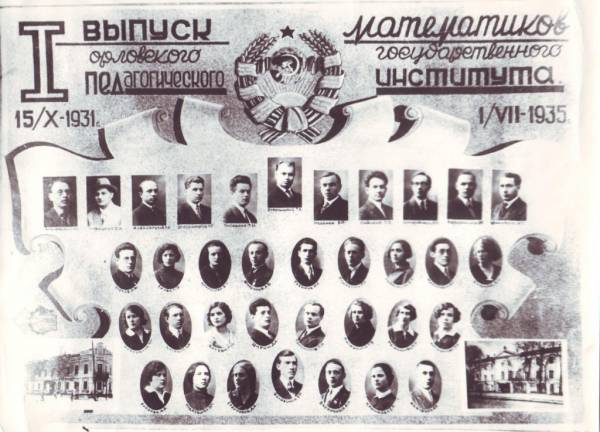
\includegraphics[scale=0.2]{1.jpg}\\
Рис. 1 - Первые преподаватели}
\end{figure}

\end{frame}

\begin{frame}
\frametitle{Факультет в годы Великой Отечественной войны}
\tiny{

Особенностью учебного процесса в послевоенный период стало то, что часть студентов пришла на факультет с фронта – завершить начатое в 30-х обучение, либо поступить на 1 курс. Учились такие парни, как правило, на «отлично». Среди них были Копаев Владимир Антонович, Парнасский Иван Васильевич. Сталинскими стипендиатами в 1947–49 годы были Иножарский Вениамин Константинович и Ростовцев Николай Михайлович. После выпуска они работали преподавателями физико-математического факультета. Алексеев Алексей Петрович окончил физмат в 1948 году, в 1953 году возглавил его как декан.
.}
\begin{figure}[!h]
\centering
\center{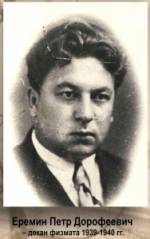
\includegraphics[scale=0.5]{2.1.jpg}
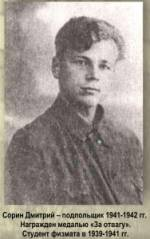
\includegraphics[scale=0.5]{2.2.jpg}\\
Рис. 2 - Преподаватели/студенты в годы Великой Отечественной войны}
\end{figure}

\end{frame}
\begin{frame}
\frametitle{Послевоенное время}
\tiny{
В 1957 году 30 июля было сдано в эксплуатацию новое здание педагогического института на улице Комсомольская, 95. Физико-математический факультет занял 4-й этаж. До сегодняшнего дня факультет адреса не изменил.Во второй половине 1980-х годов наращивался темп компьютеризации учебного процесса на факультете. Так, в 1989 году физмат получил 10 новых компьютеров марки IBM. На факультете их стало 18. Была оборудована компьютерная аудитория на первом этаже – 132-я.

Основным событием первой половины 1990-х годов стало преобразование Орловского государственного педагогического института в Орловский государственный педагогический университет (1994 г.).В 1996 году Орловский государственный педагогический университет преобразован в Орловский государственный университет.

.}
\begin{figure}[!h]
\centering
\center{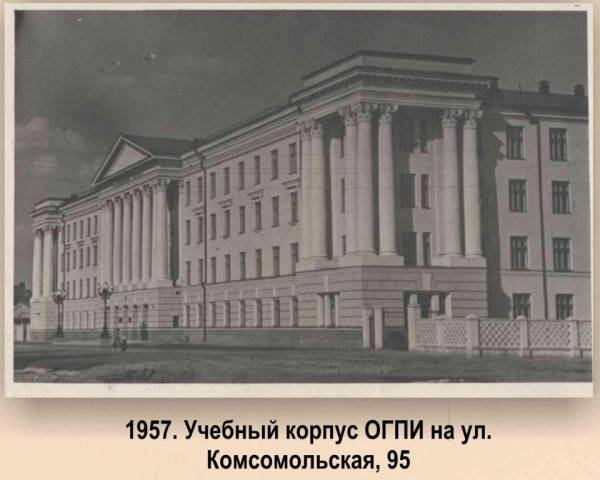
\includegraphics[scale=0.3]{3.jpg}\\
Рис. 3 - Здание педагогического института}
\end{figure}


\end{frame}
\begin{frame}

\frametitle{Корпуса}

\begin{table}[h]\begin{center}
\scalebox{0.6}{

\begin{tabular}{|c|c|}

\hline
{ 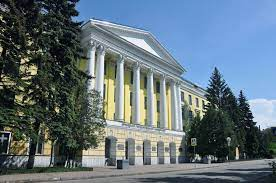
\includegraphics[scale=0.4]{glav.jpeg}} & 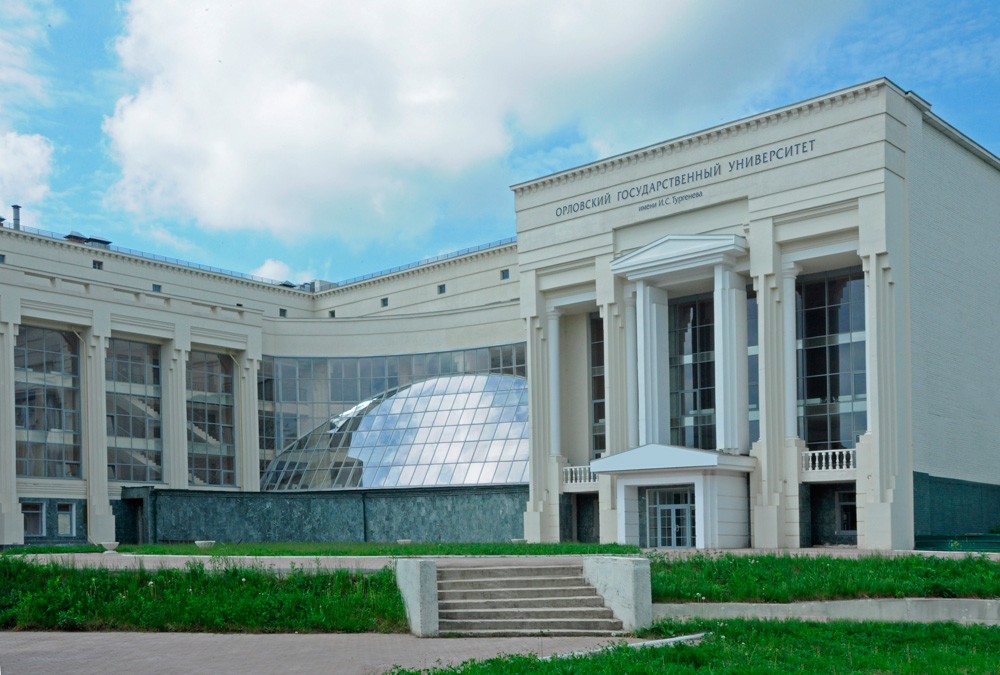
\includegraphics[scale=0.1]{bibl.jpeg} \\ \hline
\multicolumn{1}{|c|}{Корпус №1} & \begin{tabular}[c]{@{}c@{}}фундаментальная библиотека\end{tabular} \\ \hline
{ 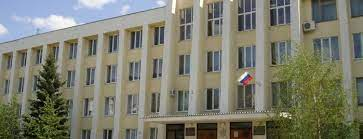
\includegraphics[scale=0.4]{3.jpeg}} & { 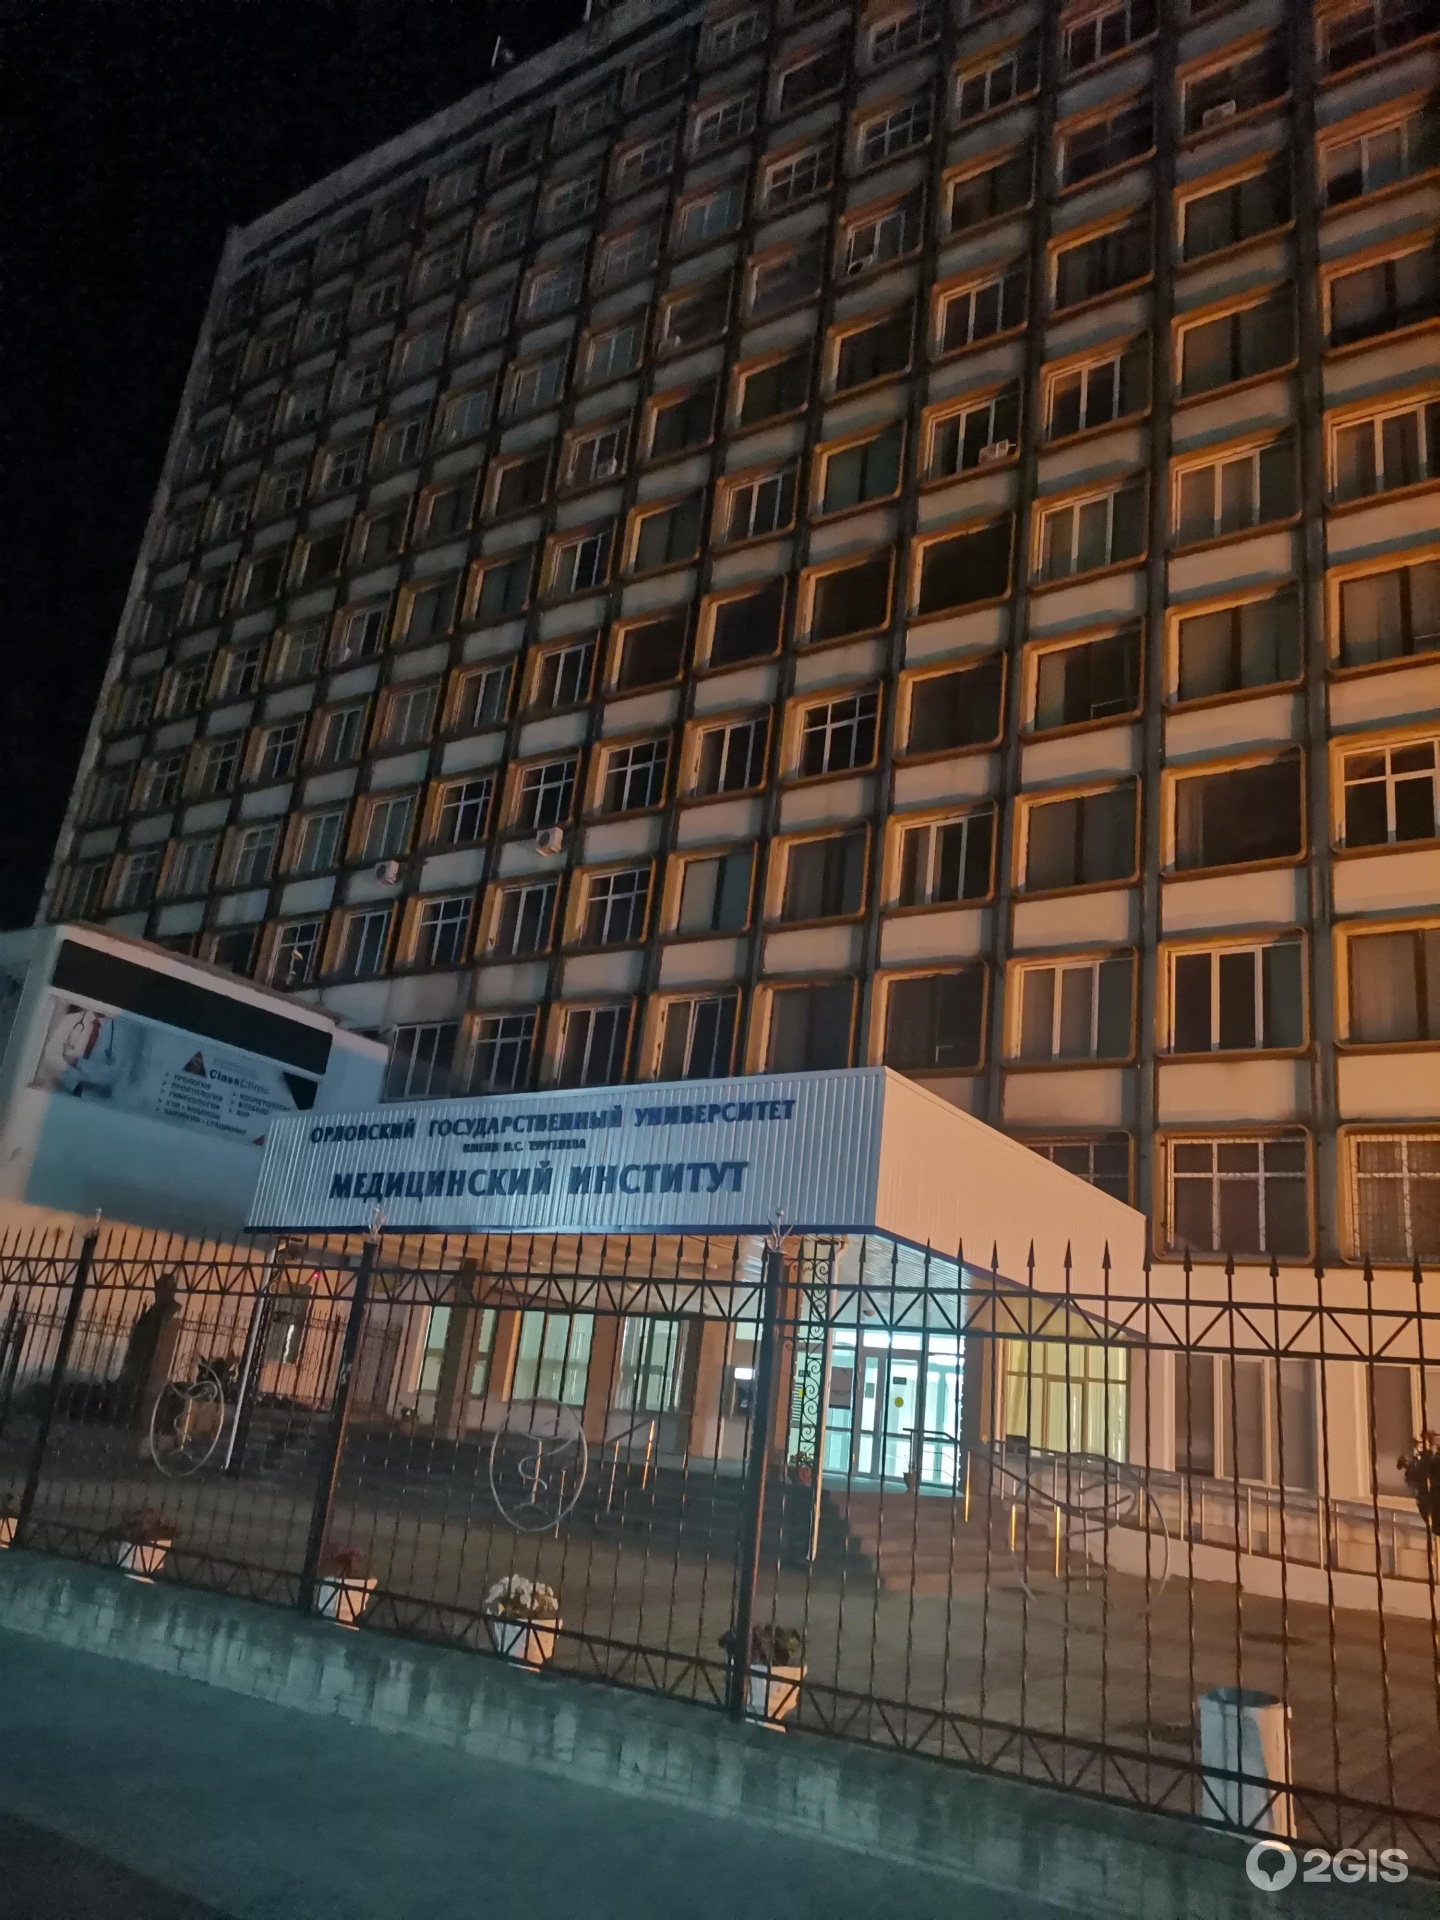
\includegraphics[scale=0.06]{nauch.jpg}} \\ \hline
Корпус №3 & \begin{tabular}[c]{@{}c@{}}Корпус №5\end{tabular} \\
\end{tabular}}
\end{center}
\end{table}

\end{frame}

\begin{frame}
\frametitle{В настоящее время}
\tiny{


Обучение студентов осуществляется по следующим направлениям бакалавриата и магистратуры: 01.03.01, 01.04.01 Математика, 01.03.02, 01.04.02 Прикладная математика и информатика, 03.03.02, 03.04.02 Физика, 44.03.05, 44.04.01 Педагогическое образование, 09.03.03, 09.04.03 Прикладная информатика.

Выпускники факультета востребованы на рынке труда и находят себе работу в самых разных организациях и учреждениях.
.}
\begin{figure}[!h]
\centering
\center{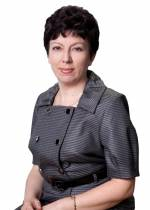
\includegraphics[scale=0.4]{4.jpg}\\
Рис. 4 - Декан факультета, кандидат физико-математических наук, профессор Т.Н. Можарова}
\end{figure}

\end{frame}


\end{document}




\fontsize{14}{18}\selectfont
\thispagestyle{empty}
\newpage
\tableofcontents
\newpage

\section{Набор формул}

\begin{center}
{\bf Степени и индексы}
\end{center}

\noindent $\blacktriangleright$ Набор в \LaTeX:
\begin{lstlisting}
$$
R_{i,j}^{k,n}
$$
\end{lstlisting}

\noindent $\blacktriangleright$ На печати 
$$
R_{i,j}^{k,n}
$$

\begin{center}
{\bf Дроби}    
\end{center}

\noindent $\blacktriangleright$ Набор в \LaTeX:
\begin{lstlisting}
$$
\frac{1}{2}, 
\frac{1}{1+\frac{1}{2}}
$$
\end{lstlisting}
\noindent $\blacktriangleright$ На печати 
$$
\frac{1}{2}, \frac{1}{1+\frac{1}{2}}
$$

\noindent $\blacktriangleright$ Набор в \LaTeX:
\begin{lstlisting}
$$
\dfrac{1}{2}, 
\dfrac{1}{1+\dfrac{1}{2}}
$$
\end{lstlisting}
\noindent $\blacktriangleright$ На печати 
$$
\dfrac{1}{2}, \dfrac{1}{1+\dfrac{1}{2}}
$$

\begin{center}
{\bf Скобки переменного размера}    
\end{center}

\noindent $\blacktriangleright$ Набор в \LaTeX:
\begin{lstlisting}
$$
\left.
\left(T
\right) \dfrac{1}{2}
\right)
$$
\end{lstlisting}

$$
\left.
\left(T
\right) \dfrac{1}{2}
\right)
$$



Корни
$$
\sqrt{4}
$$

Штрифи и многоточия
$$
f''
$$
$$
\ldots \cdots \vdots \ddots 
$$

Имена математических функций
$$
\sin() \cos() \tanh \log_{10}{2} \ln
$$
Греческий алфавит
$$\alpha, \beta \Sigma \sigma \epsilon \varepsilon$$
Символы
$$
\diamond
\blacktriangleleft
$$

Операции с пределами и без
$$
\left.\int\limits_{-\infty}^{+\infty} \sin() \, dx = -\cos(x)\right|_{a}^{b}
$$
$$
\sum\limits_{i=1}^{n}
$$

Нумерация формул
\begin{equation} \label{eq2}
\cos(x)    
\end{equation}

\begin{verbatim}
\begin{equation*} 
\sin(x)    \leqno{(**)}
\end{equation*}
\end{verbatim}


\begin{equation*} 
\sin(x) \leqno{(**)}
\end{equation*}

\begin{equation*} 
\cos(x)  \eqno{(12)}  
\end{equation*}

Включение текста в формулы \eqref{eq2}

\begin{center}
Надстрочные символы
\end{center}
$$
\overline{1,k}, \quad
\hat{x} \quad
\widehat{AB} \quad
\overrightarrow{AB}
$$
Для набора матриц используются следующие окружения:
$$
\begin{pmatrix}
a_{11} & a_{12} & \ldots & a_{1n}\\
a_{21} & a_{22} & \ldots & a_{2n}\\
\vdots & \vdots & \ddots & \vdots \\
a_{n1} & a_{n2} & \ldots & a_{nn}
\end{pmatrix}
$$

$$
\begin{vmatrix}
a_{11} & a_{12} & \ldots & a_{1n}\\
a_{21} & a_{22} & \ldots & a_{2n}\\
\vdots & \vdots & \ddots & \vdots \\
a_{n1} & a_{n2} & \ldots & a_{nn}
\end{vmatrix}
$$

\begin{equation*} 
\sin(x)    \leqno{(**)}
\end{equation*}

$$
\left(
\begin{array}{cccc}
a_{11} & a_{12} & \ldots & a_{1n}\\
a_{21} & a_{22} & \ldots & a_{2n}\\
\vdots & \vdots & \ddots & \vdots \\
a_{n1} & a_{n2} & \ldots & a_{nn}
\end{array}
\right)
$$
\parbox{75 mm}{\begin{multline} 
1+2+3+4+5+ \\
+6+7+8+ \\
 +9+10 = 45. 
\end{multline}}
\parbox{75 mm}{\begin{multline} 
1+2+3+4+5+ \\
+6+7+8+ \\
 +9+10 = 45. 
\end{multline}}

Многострочные выключные формулы

\begin{multline*} 
1+2+3+4+5+ \\
+6+7+8+ \\
 +9+10 = 45. 
\end{multline*}

\begin{gather} %\notag
1+2=3, \notag \\
1+4=5, \\
100+101 = 201.
\end{gather}

\begin{align}  %\notag
1+2=3, \\
1+4=5, \notag \\
100+101 = 201.
\end{align}


\begin{equation}
\begin{split}
1999&=1000+900+{}\\
&+90+9
\end{split}
\end{equation}

\begin{align}
7\times 9& =63 & 63:9& =7\\
9\times 10& =90 & 90:10& =9
\end{align}


Пробелы в формулах вручную \\
\begin{tabular}{|c|c|c|}
\hline
Синтаксис в \LaTeX & Комментарий & Примеры \\ \hline
\begin{lstlisting}
$x\quad y$
\end{lstlisting}
& Пробел в 1em
& $x\quad y$ \\ \hline
\begin{lstlisting}
$x\qquad y$
\end{lstlisting}
& Пробел в 2em
& $x\qquad y$ \\ \hline
\begin{lstlisting}
$\int\sin(x)dx$
\end{lstlisting}
& Без пробела
& $\int\sin(x)dx$\\ \hline
\begin{lstlisting}
$\int\sin(x)\!dx$
\end{lstlisting}
& Отрицательный пробел
& $\int\sin(x)\!dx$\\ \hline
\begin{lstlisting}
$\int\sin(x)\,dx$
\end{lstlisting}
& Тонкий пробел
& $\int\sin(x)\,dx$\\ \hline
\begin{lstlisting}
$\int\sin(x)\:dx$
\end{lstlisting}
& Средний пробел
& $\int\sin(x)\:dx$\\ \hline
\begin{lstlisting}
$\int\sin(x)\;dx$
\end{lstlisting}
& Толстый пробел
& $\int\sin(x)\;dx$\\ \hline
\end{tabular}

Листинги

\begin{lstlisting}
\begin{equation}
\begin{split}
1999&=1000+900+{}\\
&+90+9
\end{split}
\end{equation}
\end{lstlisting}

\section{Набор текста}

\section{Верстка таблиц}

\section{Подготовка презентаций}

\end{document}

